\chapter{IRRADIANCE NETWORK FORECASTS}
\label{chap:network}

With data from the irradiance monitoring network described in
\cref{chap:sens_net}, we studied a technique to produce forecasts for
one minute to one hour in advance based on the work of
\cite{Lonij2013}.
We call this forecast technique a network forecast.
Preliminary work on this is described in \cref{app:pvsc40} and an in
depth study of these types of forecasts is described in
\cref{app:network}.

The basic idea behind the network forecasts is that if a sensor
records the irradiance at some point that sensor should have some
predictive power of the irradiance for a sensor or PV power plant
downstream.
An illustration of this type of prediction is shown in
\cref{fig:leading_sens} where the output of sensor 19 predicts the
output of sensor 31 with an eight minute lead time.

\begin{figure}[bht]
\centering
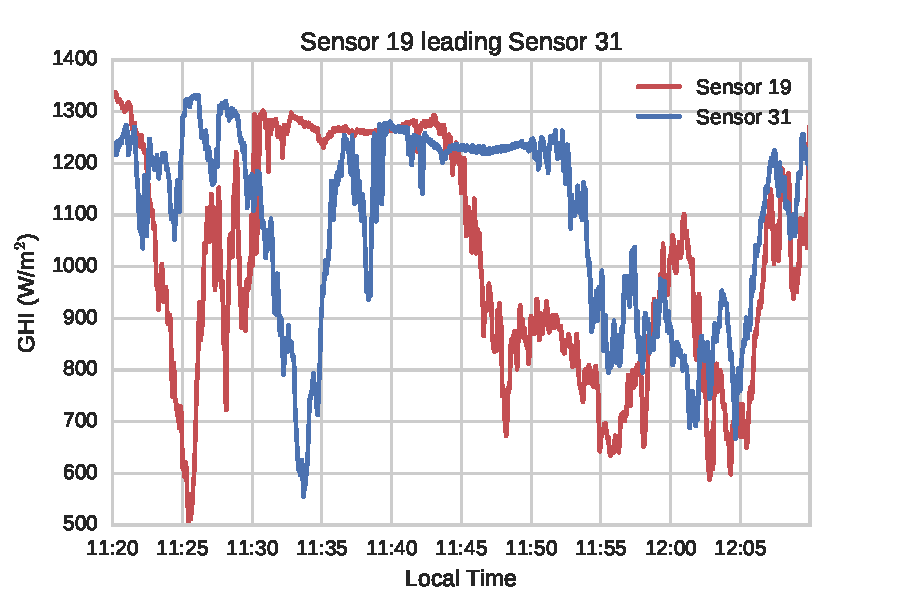
\includegraphics[width=.8\textwidth]{figs/leading_sens.pdf}
\caption[Example of data from one sensor predicting the output of
another]{An example of the output of sensor 19 (red) predicting what
  the output of the upstream sensor 31 (blue) in roughly 8
  minutes.}
\label{fig:leading_sens}
\end{figure}

\section{Irradiance Forecast Error Metrics}
\label{sec:error_metrics}

While studying and evaluating the forecasts described in
\cref{app:network}, we learned how important it is to understand
forecast error metrics and their limitations.
Here we present an examples of possibly misleading error metrics as a
warning to those evaluating forecasts to exercise care.

We will evaluate each metric on forecasts of clear-sky index to remove
the time of day weighting that is implicit when computing errors for
GHI.
First, we will define the error metrics to be discussed.
The most common metrics are mean bias error (MBE), mean absolute error
(MAE), and root mean squared error (RMSE) that are defined as
\begin{equation}
\mbox{MBE} = \frac{1}{N} \sum_{i=0}^N (f_i - o_i),
\end{equation}
\begin{equation}
\mbox{MAE} = \frac{1}{N} \sum_{i=0}^N |f_i - o_i|,
\end{equation}
\begin{equation}
\mbox{RMSE} = \sqrt{\frac{1}{N} \sum_{i=0}^N (f_i - o_i)^2},
\end{equation}
where $f_i$ is the forecast at time $i$ and $o_i$ is the observation
of a sensor.
MBE indicates the average bias of a forecast, and if it is not nearly
zero, bias correction techniques may be applied to the forecast to
reduce it further.
MAE indicates the average magnitude of errors as does RMSE, but RMSE
weights large errors more.
Other metrics and examples of their use can be found
in~\cite{Zhang2015,Jensen2016}.

Other metrics include Pearson's correlation coefficient, the standard
deviation of the errors, and the standard deviation of the forecasts
as compared to the standard deviation of the observations.
A number of other possible useful metrics are defined
in~\cite{Zhang2015}.
We will also look at the ramp metrics defined in~\cite{Chu2015b}, the
ramp detection index (RDI), false ramp index (FRI), and ramp
magnitude forecast index (RMI).

\subsection{Example Forecasts}
Here we present forecasts for two days in Tucson, AZ, in 2014.
The first day shown in \cref{fig:5minfx_day1} has thick but broken
clouds.
The second day shown in \cref{fig:5minfx_day2} has more scattered
clouds.
In each case, observations are averaged to five minutes, Forecast A is
a five minute persistence forecast, Forecast B is a smoothing applied
to the data, and Forecast C is a fraction of the clear-sky profile for
that day.

\begin{figure}[tbp]
\centering
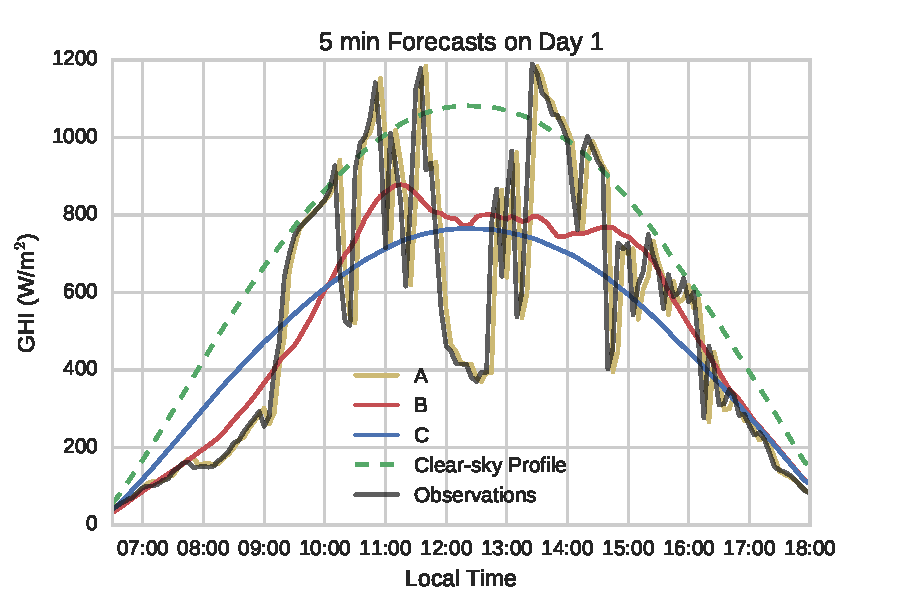
\includegraphics[width=0.8\textwidth]{figs/error_fx_Day_1.pdf}
\caption[Forecasts for a day with thick, broken clouds]{Five minute
  ahead forecasts for a day with thick broken clouds. Forecast A is a
  persistence forecast that captures the variability of the
  observations, but offset by 5 minutes. Forecast B is a somewhat
  smoothed forecast, and Forecast C is simply a fraction of the
  clear-sky profile.}
\label{fig:5minfx_day1}
\end{figure}

\begin{figure}[tbp]
\centering
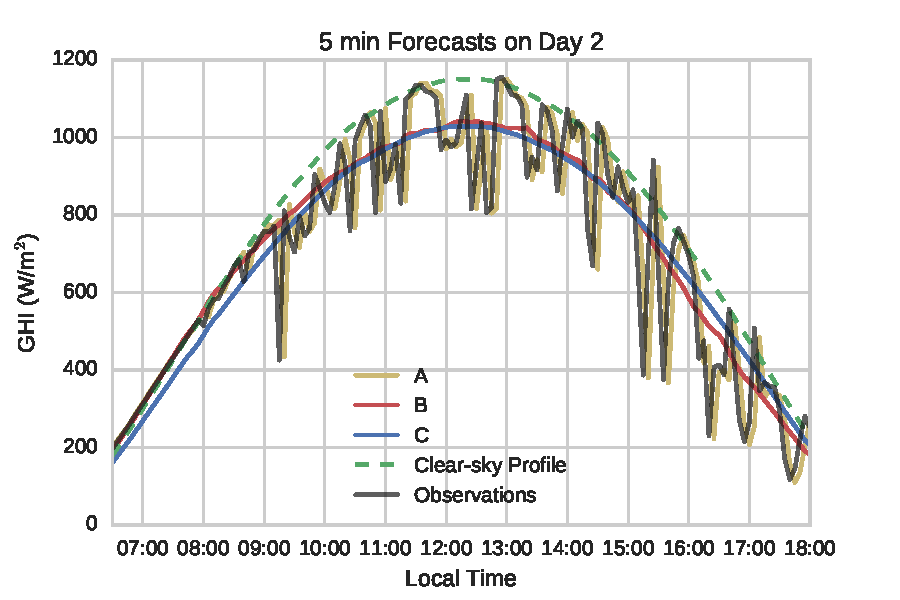
\includegraphics[width=0.8\textwidth]{figs/error_fx_Day_2.pdf}
\caption[Forecasts for a day with scattered clouds]{Five minute
  ahead forecasts for a day with scattered clouds. Forecast A is a
  persistence forecast that captures the variability of the
  observations, but offset by 5 minutes. Forecast B is a somewhat
  smoothed forecast, and Forecast C is simply a fraction of the
  clear-sky profile.}
\label{fig:5minfx_day2}
\end{figure}

Which forecast is best depends on how one plans to use the forecast.
If one is concerned with quanities like average hourly production from
a PV plant, perhaps the smoother Forecast B is best.
If one is concerned with variability to, for example, schedule
generation to back up solar power, Forecast A might be preferable.
In most cases, Forecast A is considered the better forecast that
better captures the nature of the observations.

\Cref{table:fx_errs} shows the values of some standard error metrics
for forecasts on each day.
For Day 1, Forecast A is clearly the best forecast with the lowest
MAE and RMSE, and the highest correlation to the observations.
It also performs better at detecting ramp events.
On Day 2, MAE and RMSE would suggest that Forecast B is the best.
Furthermore, Forecast C has the same RMSE as Forecast A.

\begin{table}[htbp]
\centering
\caption[Error metrics for contrived test forecasts]{Error metrics (in units
of clear-sky index) for the forecasts on Day 1 shown in
\cref{fig:5minfx_day1} and Day 2 shown in
\cref{fig:5minfx_day2}. Refer to the text of \cref{sec:error_metrics}
for a description of each metric.}
\label{table:fx_errs}
\vspace{.3em}
\captionsetup{position=top}
\subfloat[Day 1\label{table:fx_errs_day1}]{\input{figs/Day_1_err_table}}
\hspace{3em}
\subfloat[Day 2\label{table:fx_errs_day2}]{\input{figs/Day_2_err_table}}
\end{table}

If given Forecast B or C on Day 2, a user might consider it to be a
forecast of a clear day, although with possibly more aerosols in the
air reducing the irradiance slightly from the expected clear-sky
profile.
Forecast A is the only forecast to capture the variability that is
also seen in the observations and is often most concerning to
utilities.
Thus, the metrics are somewhat misleading on Day 2.

\subsection{Taylor Diagrams}
The Taylor diagram is an execellent tool to summarize a number of
metrics for many forecasts in a single figure \citep{Taylor2001}.
\Cref{fig:taylor_day1,fig:taylor_day2} are the Taylor diagrams for the
forecasts on Day 1 and Day 2, respectively.
For any forecast, the radius indicates the standard deviation of the
forecast and the angle is the correlation of the forecast with the
observations.
The gray contours indicate lines of constant centered RMSE, or RMSE
once any bias has been removed from the forecast.
A perfect forecast would lie on the x-axis (correlation = 1) and have
the same standard deviation as the observations.

\begin{figure}[p]
\centering
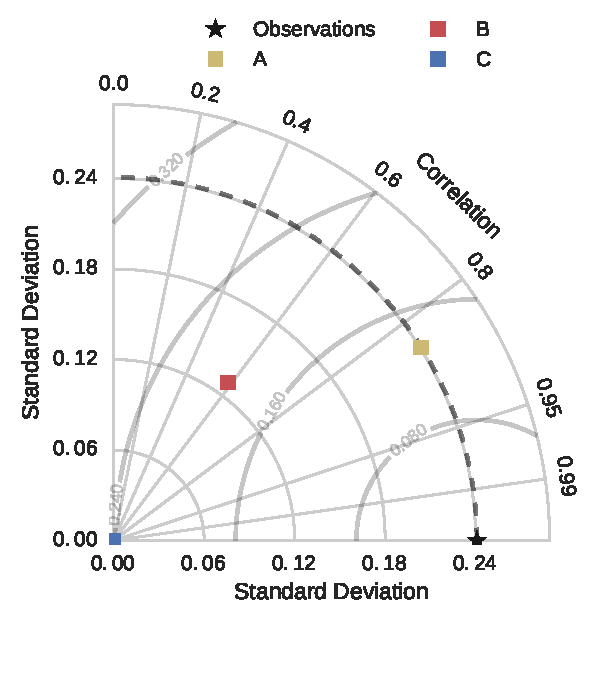
\includegraphics[width=0.8\textwidth]{figs/taylor_Day_1.pdf}
\vspace{-3em}
\caption[Taylor diagram for day 1 example forecasts]{A Taylor diagram
  for the forecasts on Day 1 shown in \cref{fig:5minfx_day1}. The
  light gray contours are lines of constant CRMSE. Forecast A has the
  lowest CRMSE in addition to having the same variability, as measured
  by the standard deviation, as the observations.}
\label{fig:taylor_day1}
\end{figure}

\begin{figure}[p]
\centering
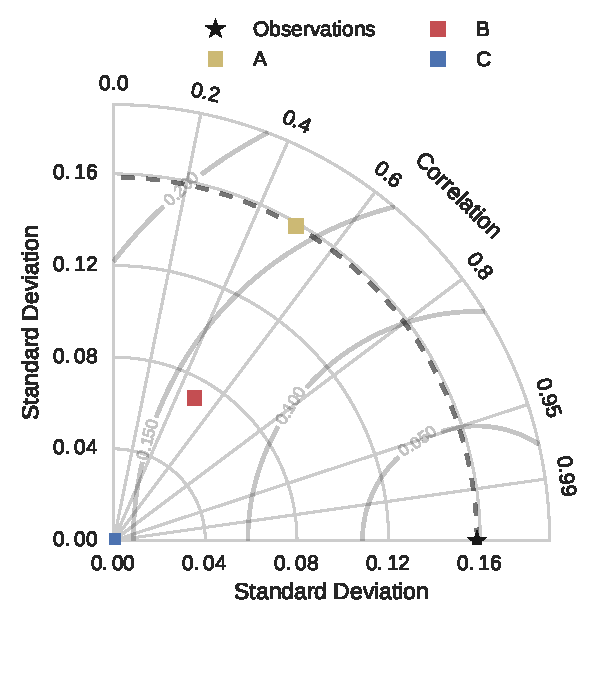
\includegraphics[width=0.8\textwidth]{figs/taylor_Day_2.pdf}
\vspace{-3em}
\caption[Taylor diagram for day 2 example forecasts]{A Taylor diagram
  for the forecasts on Day 2 shown in \cref{fig:5minfx_day2}. On this
  day, Forecast B has a smaller CRMSE and about the same correlation
  as Forecast A. However, Forecast A has similar variability to the
  observations as measured by the standard deviation. Depending on
  what the intended use of the forecast is, Forecast A may be the
  ``better'' forecast.}
\label{fig:taylor_day2}
\end{figure}

\Cref{fig:taylor_day1} confirms our assessment that Forecast A is best
on Day 1 since it has the lowest CRMSE, standard deviation equal to
that of the observations, and the highest correlation to the
observations.
From \cref{fig:taylor_day2}, Forecast A is better than Forecast C
since they have a similar CRMSE but Forecast A actually matches the
variability observed in the observations.
On the other hand, Forecast B has a lower CRMSE, but does not capture
this variability.
In this case, it depends on the use case to say whether Forecast A or
Forecast B is best.

\subsection{Suggestions}
We have hopefully demonstrated why an understanding of the error
metrics and careful application is important when evaluating
forecasts.
Evaluating forecasts on only a single or a couple of days may lead to
conflicting results, so a longer time period with varied weather
should be used when considering the overall performance of a forecast.
Furthermore, a number of metrics should be calculated and compared to
 understand the differences in forecasts, and the Taylor diagram
provides a good summary of some metrics.
Finally, an examination of the actual forecast as compared to
observations is useful to gain an intuitive sense of the forecast.

When comparing errors across studies, it is important to also consider
the region that the forecast was made for.
For example, the desert Southwest experiences fewer overcast days than
locations in the Southeast.
The Southwest also has a high number of clear days.
A forecast with low errors in the Southeast may be better at
forecasting overcast days with less skill on mostly clear days.

\section{Future Work}
One limitation to the network forecast methodology that we studied is
that only a single velocity vector was used to transport the predicted
clear-sky index map.
Future work could explore using a number of vectors based on clouds at
different heights and a proper advection scheme.
One might also explore which domains this type of forecast performs
best in order to switch between forecast methodolgies for different
domains.
Future work that may overcome the issue of clear-sky index maps
generated in \cref{app:network} not resembling reality by using
satellite cloud estimates will be described in \cref{chap:satfx}.


%%% Local Variables:
%%% mode: latex
%%% TeX-master: "dissertation"
%%% End:
